\section{Parte 02 – MODELO CANVAS DEL "RESTAURANTE EL CACIQUE"} 

\begin{enumerate}[1.]
	\item \textbf {PASO 1: LIENZO DE MODELO DE NEGOCIO} \newline
\begin{center}
\textbf {SOCIOS CLAVE} \newline
\end{center}
Proveedores: \newline
* Suministro constante y oportuno que ayudaran con el abastecimiento de nuestro local (embutidos, carnes, bebidas embotelladas, productos de limpieza, envases, etc) \newline
* La Genovesa, distribuidora de bebidas.\newline
\\ 
\begin{center}
\textbf {ACTIVIDADES CLAVE} \newline
\end{center}

* Elaboracion de productos de manera rapuda y de calidad, tales como pollo brasther, picante a la tacneña, lomo saltado, etc.\newline
* Buena atencion a los clientes.\newline
* Uso del libro de sugerencias para mejorar nuestro negocio.\newline
* Satisfaccion de los clientes.\newline
\\ 
\begin{center}
\textbf {RECURSOS CLAVE} \newline
\end{center}

* Capital por parte de los socios\newline
* Local \newline
* Personal capacitado para la elaboracion. distribucion, compra, venta y atencion.\newline
* Materias primas para la elaboracion del producto.\newline
* Mantenimiento del local.\newline
* Servicios de agua, luz.\newline

\item \textbf {PASO 2: PROPUESTA DE VALOR} \newline
\\
* Brindar al cliente productos de manera rapida\newline
* Sabores exquisitos y de calidad\newline
* A un  buen precio de acuerdo al bolsillo de nuestros consumidores.\newline
* Brindaremos seguridad en el local (camaras de vigilancia).\newline
* "Comida rapida de la cual te puedas sentir bien al comer", sin sentimiento de culpa.\newline
* Promociones\newline

\begin{center}
\textbf {RELACIONES CON LOS CLIENTES} \newline
\end{center}
* Relacion de asistencia personal\newline
* Relacion de autoserviciol\newline
* Relacion de comunidades\newline
\\ 

\begin{center}
\textbf {CANALES} \newline
\end{center}
* Venta directa\newline
\\ 

\begin{center}
\textbf {SEGMENTOS DE CLIENTES} \newline
\end{center}
Trabajadores, estudiantes y publico de la ciudad de tacna  \newline
\\ 
\begin{center}
\textbf {ESTRUCTURA DE COSTOS} \newline
\end{center}
*Servicios de agua y luz.  \newline
*Mantenimiento de nuestros electrodomesticos y local.  \newline
*Publicidad y mercadeo.  \newline
*Sueldos.  \newline
\\ 

\begin{center}
\textbf {FUENTES DE INGRESO} \newline
\\
\end{center}
La contribucion a los ingresos totales por parte de los productos  \newline
\\ 

	\begin{center}
	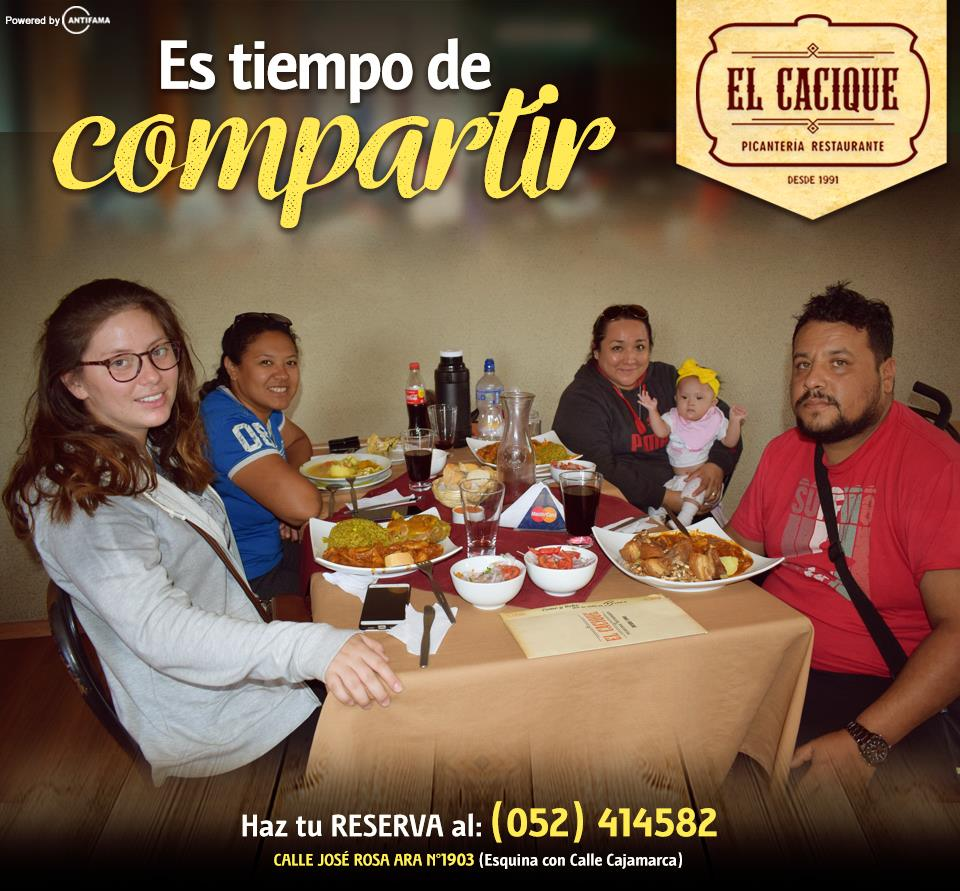
\includegraphics[width=10cm]{./Imagenes/clientes} 
	\end{center}

	\begin{center}
	\includegraphics[width=10cm]{./Imagenes/ clientes2} 
	\end{center}



\end{enumerate} 
